\documentclass{article}
\usepackage{amsmath,amssymb}
\usepackage{latexsym}
\usepackage{diagbox}
\usepackage{graphicx}
\usepackage{color}
\usepackage{bm}
\usepackage{ulem}
\usepackage{float}
\usepackage{subfigure}
\usepackage{listings}
\lstset{
	frame=lrtb
	breaklines=true	
}
\usepackage{pdfpages}
\begin{document}
	
	\title{Microeconometrics Assignment 3} 
	\author{Jia Ru, 27720141152749} 
	
	\maketitle
	
	
\section{Treatment Effect}
Consider the treatment-outcome model
$$ y = x\beta + \alpha d + \epsilon $$
\subsection*{(a) Is randomized treatment a sufficient condition for identification of $\alpha$ and $\beta$ ?}
Random assignment of treatment allow the identification of the ATT(Average Treatment Effect of the Treated,or TOT in some books),i.e. the parameter $\alpha$, but without further assumptions do not necessarily allow one to identify the underlying structural parameters of $\beta$.\\
To interprete it in detail, let $Y_1$ and $Y_0$ denote the outcome if the individual is treated/not treated, respectly. So only one of $Y_1$ and $Y_0$ can be observed, the other is "counterfactual". And the observed outcome $Y_i$, can be write as
$$ Y_i = d_iY_{1i} + (1-d_i)Y_{0i} $$
Define the treatment effect
$$ \alpha_i = Y_{1i}-Y_{0i} $$
And Average Treatment Effect(ATE) as well as Average Treatment Effect of the Treated(ATT)
$$ E[\alpha_i] = E[Y_{1i}-Y_{0i}] $$
$$ E[\alpha_i|d_i=1] = E[Y_{1i}-Y_{0i}|d_i=1] $$
Since
\begin{align*}
  & E[Y_i|d_i=1]-E[Y_i|d_i=0] \\
= & E[Y_{1i}|d_i=1]-E[Y_{0i}|d_i=1] + {E[Y_{0i}|d_i=1] - E[Y_{0i}|d_i=0]} \\
= & ATT+ E[Y_{0i}|d_i=1] - E[Y_{0i}|d_i=0] \\
\end{align*}
The first term is the parameter of interest, $\alpha$, the remainder is the selection bias term. In the case of random assignment of treatment, it is zero . So we can identify parameter $\alpha$. \\
But we could not identify parameter $\beta$ without the information of the correlation between $x$, $d$ and $\epsilon$. If 
$$ E[u|x]=0$$
then we can identify parameter $\beta$.

\subsection*{(b)If participation of treatment (d = 1 or 0) is correlated with y, suggest a method to obtain $\alpha$.}
We can use IV method to estimate $\alpha$: Find an inturment variable $Z$, such that $Z$ is correlated with $d$ but not correlated with $X$ or $\epsilon$, i.e. $Z$ affacts the outcome $Y$ only thouth treatment $d$.

\subsection*{(c) Suppose the outcome equation is unknown, eligibility of treatment is exogenously determined, suggest a method to obtain the average treatment effect.}

If eligibility of treatment (instead of treatment per se) is randomized, It can be proved that(the proof is omitted here):
$$ TOT\equiv E[Y_1-Y_0|d=1]=\frac{E[Y|e=1]-E[Y|e=0]}{Prob(d=1|e=1)}=\frac{ITT}{ program\ participation\ rate.} $$
where dummy $e$ denote "Eligibility", ITT means "Intent-to-Treat" effect\\
So given observed data, ATE can be estimated as: difference of sample mean of subsamples of eligible and not eligible, divided by program paricipation rate.


\section{Empirical Analysis}

\subsection{Explore the data set.Identify which variables are time variant, individual variant or both.}

\paragraph{} Group the observations by id and time, respectively. 
Then see the summary statistic of all the variables.
Analysis the tables (especially the Std.Dev. collomn) I find:\\
\begin{itemize}
	\item OCC, IND, SOUTH, SMSA, FEM, UNION, ED, BLK is invariant accross time.
	\item No variable is invariance accross id
	\item Other variables are both time variant and individual variant.
\end{itemize}

\lstset{
	basicstyle=\ttfamily,
	frame=lrtb,  %%%%%%%%% accross page?
	breaklines=true	
}

\begin{lstlisting}
	sort id
	by id: summ
	sort time
	by time:summ	
\end{lstlisting}
( results ommited, since it' too much )

\subsection{Set panel Structure. Compute summary statistics for all the variables.Are there any ‘suspicious values’?}
\begin{lstlisting}
      xtset, clear
      xtset id time
      xtdescribe
      xtsum
\end{lstlisting}

	\paragraph{} Consider the "Std.Dev." column of `xtsum` table. 
	For id, FEM, UNION, ED, BLK the within standard deviation is 0.
	Only time's between Standard deviation is 0.
	\paragraph{}  The 'suspicious values' appears for the 4 variables:
	OCC, IND, SOUTH, SMSA. The conclusion seems contradict in 1) and 2)
	After checking the meannning of these variables, 
	I speculate that it's becuase, take OCC for example, 
	a few people transfers form blue-collar occupation to other 
	occupation type during the survey years, 
	consisting a small percent of the total sample however. So I didn't
	perceive these pattern in question 1), 
	(Since this data have 595 id, I couldn't check it one by one).


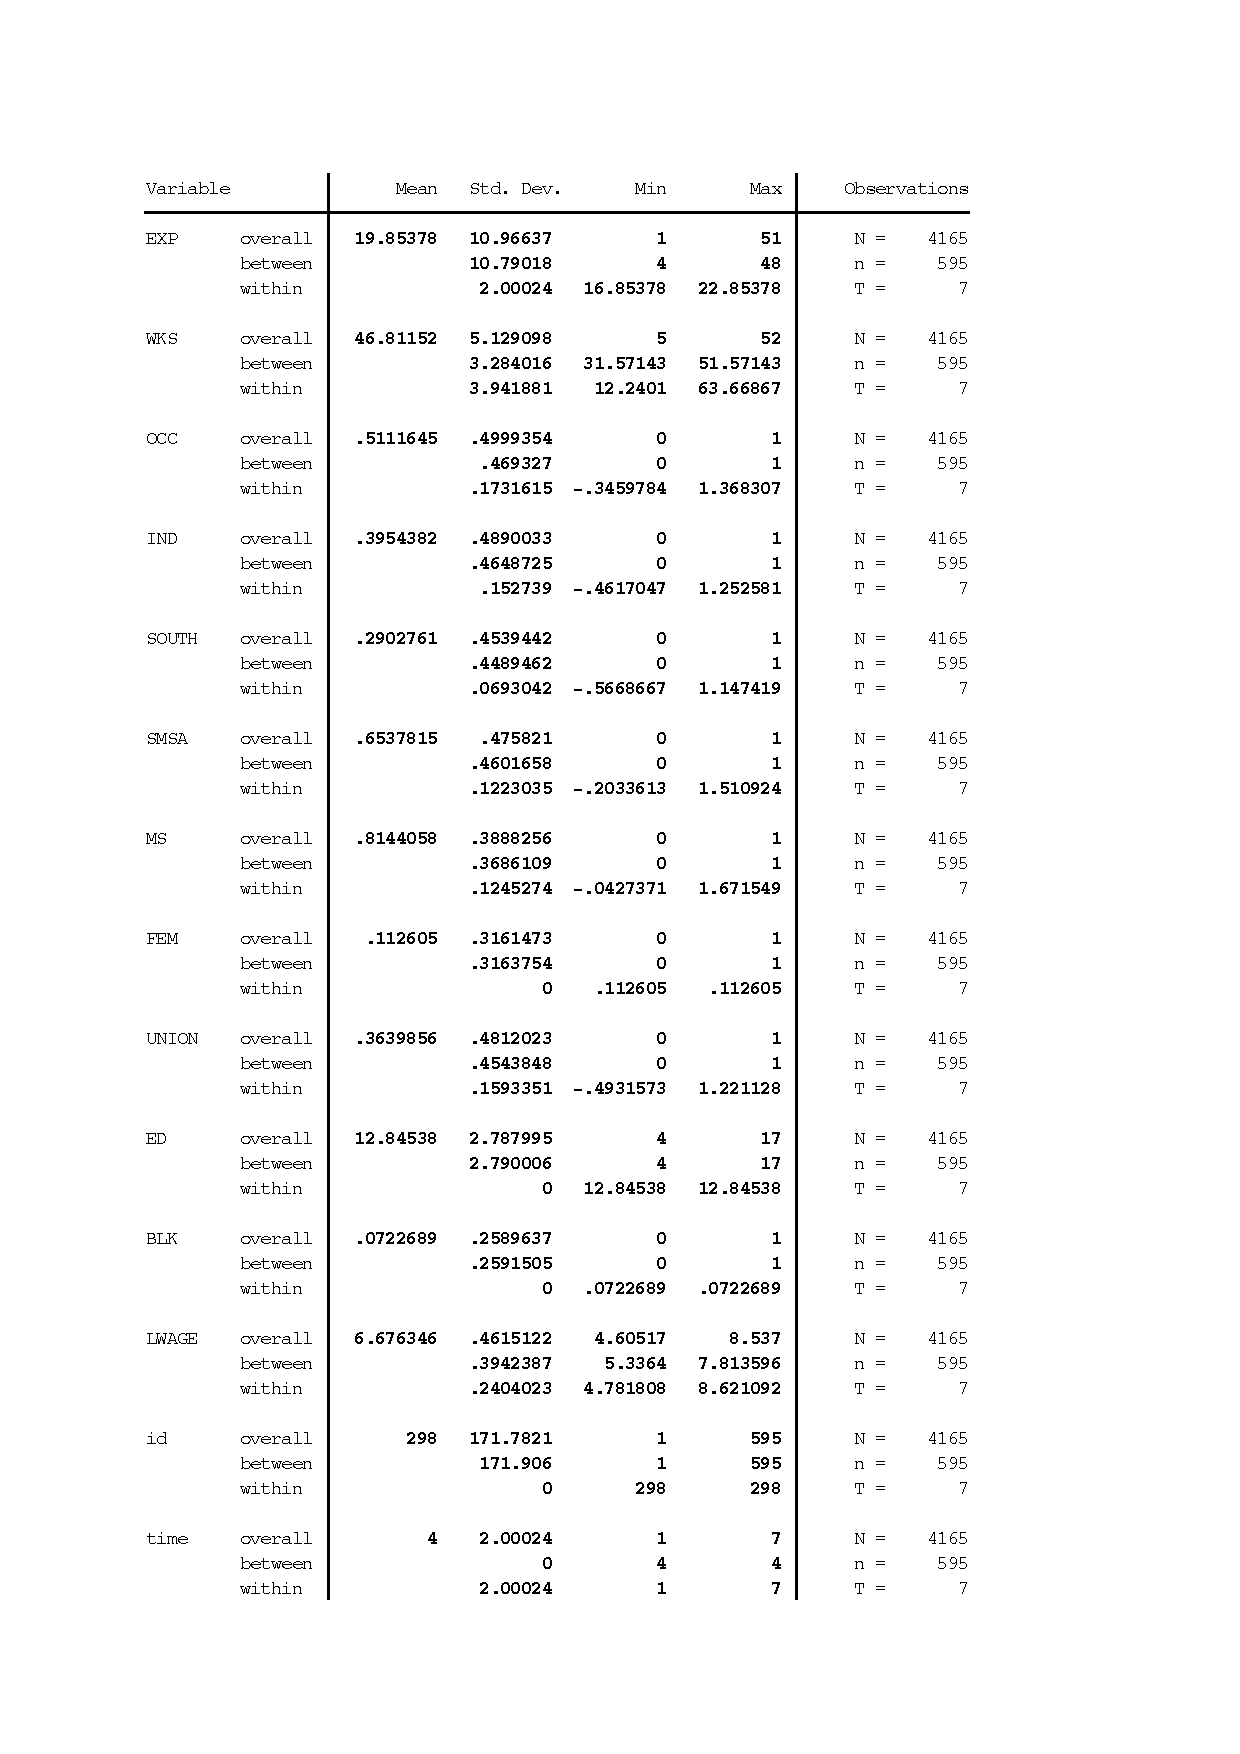
\includepdf{xtsum.pdf}


\subsection{GLS regression}
\begin{lstlisting}
    gen EXP2 = EXP*EXP
    
    global Y "LWAGE"
    global X "EXP EXP2 WKS OCC IND SOUTH SMSA MS FEM UNION ED BLK"
    
    est clear
    set matsize 595, permanently
    
    xtgls $Y $X, i(id) corr(ind) 
    est store GLS
    
\end{lstlisting}
\paragraph{ I. Do the signs of the parameters agree with your intuition? \\} 
For variable EXP: as one accumulate his working experience, his wages will increase (coef. of EXP is positive), 
however this marginal effects decrease (coef. of EXP2 is negative).\\
coefficients of other variables all agree with my intuition: 
The people who 
have more working hours and high education,
being in in a manufacturing industry, 
married,
being in Union
tends to have more wage, while people who are
black
female,
blue-collar worker, 
live in south
ends to have less wage.
\paragraph{II. What variables are significant at 5\% level? \\}  
All the variables.
\paragraph{III.Is this an appropriate procedure?\\}  
No, this pooled model do not consider heterogenity, that is to say,
it implictly assumes that different individuals have same constant 
term. There are some factors, say, people's ability, can affact WAGE,
which is unobservable, since different people have different ability,
it's unreasonable to use pooled model.

\subsection{Implement the following methods for the wage equation:}
\begin{itemize}
	\item Fixed effects (within)
	\item Random effects (GLS)
	\item Between
	\item Random effects (ML)
\end{itemize}
\begin{lstlisting}
xtreg $Y $X , fe
est store fe

xtreg $Y $X , re
est store re_GLS

xtreg $Y $X , be
est store be

xtreg $Y $X , mle
est store re_ML

outreg2 [GLS fe re_GLS be re_ML] using "tex/reg.tex" ///
, nose replace tex(frag) title("Regression Resutlts")		
\end{lstlisting}

\begin{tabular}{lccccc}
\multicolumn{6}{c}{REGRESSION RESULTS} \\ \hline
 & (1) & (2) & (3) & (4) & (5) \\
 & GLS & fe & re\_GLS & be & re\_ML \\
VARIABLES & LWAGE & LWAGE & LWAGE & LWAGE & LWAGE \\ \hline
 &  &  &  &  &  \\
EXP & 0.0401*** & 0.113*** & 0.0821*** & 0.0319*** & 0.107*** \\
EXP2 & -0.000673*** & -0.000418*** & -0.000808*** & -0.000566*** & -0.000515*** \\
WKS & 0.00422*** & 0.000836 & 0.00103 & 0.00919** & 0.000840 \\
OCC & -0.140*** & -0.0215 & -0.0501*** & -0.168*** & -0.0251* \\
IND & 0.0468*** & 0.0192 & 0.00374 & 0.0579** & 0.0138 \\
SOUTH & -0.0556*** & -0.00186 & -0.0166 & -0.0571** & 0.00577 \\
SMSA & 0.152*** & -0.0425** & -0.0138 & 0.176*** & -0.0475** \\
MS & 0.0484** & -0.0297 & -0.0746*** & 0.115** & -0.0414** \\
FEM & -0.368*** &  & -0.339*** & -0.317*** & -0.176 \\
UNION & 0.0926*** & 0.0328** & 0.0632*** & 0.109*** & 0.0387*** \\
ED & 0.0567*** &  & 0.0997*** & 0.0514*** & 0.136*** \\
BLK & -0.167*** &  & -0.210*** & -0.158*** & -0.261* \\
o.FEM &  & - &  &  &  \\
o.ED &  & - &  &  &  \\
o.BLK &  & - &  &  &  \\
Constant & 5.251*** & 4.649*** & 4.264*** & 5.121*** & 3.126*** \\
Constant & 5.251*** & 4.649*** & 4.264*** & 5.121*** & 0.839*** \\
Constant & 5.251*** & 4.649*** & 4.264*** & 5.121*** & 0.153*** \\
 &  &  &  &  &  \\
Observations & 4,165 & 4,165 & 4,165 & 4,165 & 4,165 \\
R-squared &  & 0.658 &  & 0.544 &  \\
 Number of id & 595 & 595 & 595 & 595 & 595 \\ \hline
\multicolumn{6}{c}{ Standard errors in parentheses} \\
\multicolumn{6}{c}{ *** p$<$0.01, ** p$<$0.05, * p$<$0.1} \\
\end{tabular}
	

\paragraph{Do the signs of the parameters agree with your intuition?\\}
\begin{itemize}
	\item EXP: Yes. as EXP increase, his wages will increase (coef. of EXP is positive), however this marginal effects decrease (coef. of EXP2 is negative).
	\item WKS: Yes. the coef. is positive which means more working hour, more wages.
	\item OCC: Yes. bule-collar works earn less than white-collar, it consist with intuition.
	\item IND: the regression result tells me manufacture industry earns more, maybe it's true.
	\item SOUTH, SMSA, MS: the 4 regression give different signs of coefficient.
	\item FEM: Yes, Even in the U.S, female earn less than male, it's also the case in China.
	\item UNION: Yes, being in the Union will have more wage, since they have more bargining power.
	\item EDU: Yes, Education attainment and wages is positively-correlated, Substaintial number of literatures in Labor Economic have studied this issue.
	\item BLK: Yes, people who are black earns less, whether it's due to race discrimination or ability which is unobervable, howerver, is not clear.
\end{itemize}
\paragraph{What variables are significant at 5\% level?\\}
\begin{itemize}
	\item fe: EXP SMSA UNION
	\item re-GLS: EXP OCC MS FEM UNION ED BLK
	\item be: All varibles
	\item re-ML: EXP OCC SMSA MS UNION ED BLK
\end{itemize}
\paragraph{Is the estimation procedure appropriate for the context?Is the estimator consistent? Compare the results. Do you accept or reject the presence of individual effects? Why or why not?\\}
The estimation of panel data models boils down to the choice between three estimators:\\
1. The pooled model should be used when there is no individual heterogeneity in the model.\\
2. When there is individual heterogeneity and it is not correlated with the independent variables of the model, the random effects model should be preferred. The Hausman test helps us decide
whether this is the case or not. \\
3. If the individual heterogeneity is correlated with the independent variables, the fixed effects model should be used.\\
In this context, the dependent variable is WAGE, by intuition, we can not ignore heterogeneity, since different people have different abiliy, characterictics, pereferences and so on, these factors will affect WAGE and it varies accross individuals. The poold regression model is not reasonable.\\
So the pooled model in collumn 1 is not consistent, the fixed effect model in column 2,4 is always consistent, at the expense of efficiency. Whether random effect model is consistent depends on whether the assumption of random effect model are satisfied, which will disscuss later, if true, the random effect model is alse consistent as well as efficient(than fixed effect model).

\subsection{Compute the estimates of specific effects (fixed and random). Comment. Would you prefer the fixed effects or the random effects results? Why? (you can use the Hausman test).}
\paragraph{} Panel data models acknowledge that different units behave differently by adding an individual heterogeneity term.There are two kinds of panel data models that account for individual heterogeneity in two different ways: fixed effects model and random effects model. Fixed effects model assumes that the heterogeneity term and the independent variables x are correlated, while random effects model assumes that the heterogeneity term and the independent variables x are not correlated.
\paragraph{} In this wage equaiotn context, I think fixed effects model is better. Because here the heterogeneity term is correlated with the X's. for example, individual's ability or characteristic or working-leisure pereferance affacts his wage, and it's self-evident that people's ability is correlated with his education attainment. This reasoning is based on economic intuition. Also we should apply Statistic method to see if the assumption of random effect model holds, that is, Hausman Test:
\begin{lstlisting}
    hausman fe re_GLS 
\end{lstlisting}

\begin{lstlisting}[basicstyle=\footnotesize\ttfamily]
---- Coefficients ----
(b)          (B)            (b-B)     sqrt(diag(V_b-V_B))
fe         re_GLS       Difference          S.E.

EXP	     .1132083     .0820544        .0311539               .
EXP2     -.0004184    -.0008084        .0003901               .
WKS	     .0008359     .0010347       -.0001987               .
OCC	     -.0214765    -.0500664        .0285899               .
IND      .0192101     .0037441         .015466               .
SOUTH    -.0018612    -.0166176        .0147564        .0217436
SMSA     -.0424692    -.0138231       -.0286461               .
MS	     -.0297258    -.0746283        .0449025               .
UNION    .0327849     .0632232       -.0304384               .

b = consistent under Ho and Ha; obtained from xtreg
B =	inconsistent under Ha, efficient under Ho; obtained from xtreg

Test:  Ho:	difference in coefficients not systematic

chi2(9) = (b-B)'[(V_b-V_B)^(-1)](b-B)
=     5075.25
Prob>chi2 =      0.0000
(V_b-V_B is not positive definite)
\end{lstlisting}
Because the p-value is very small(Prob$>$chi2 =0.0000), which means that the we should reject H0, that is, use the fixed effect model.


\section{Question 3}

\begin{figure}[H]
\centering
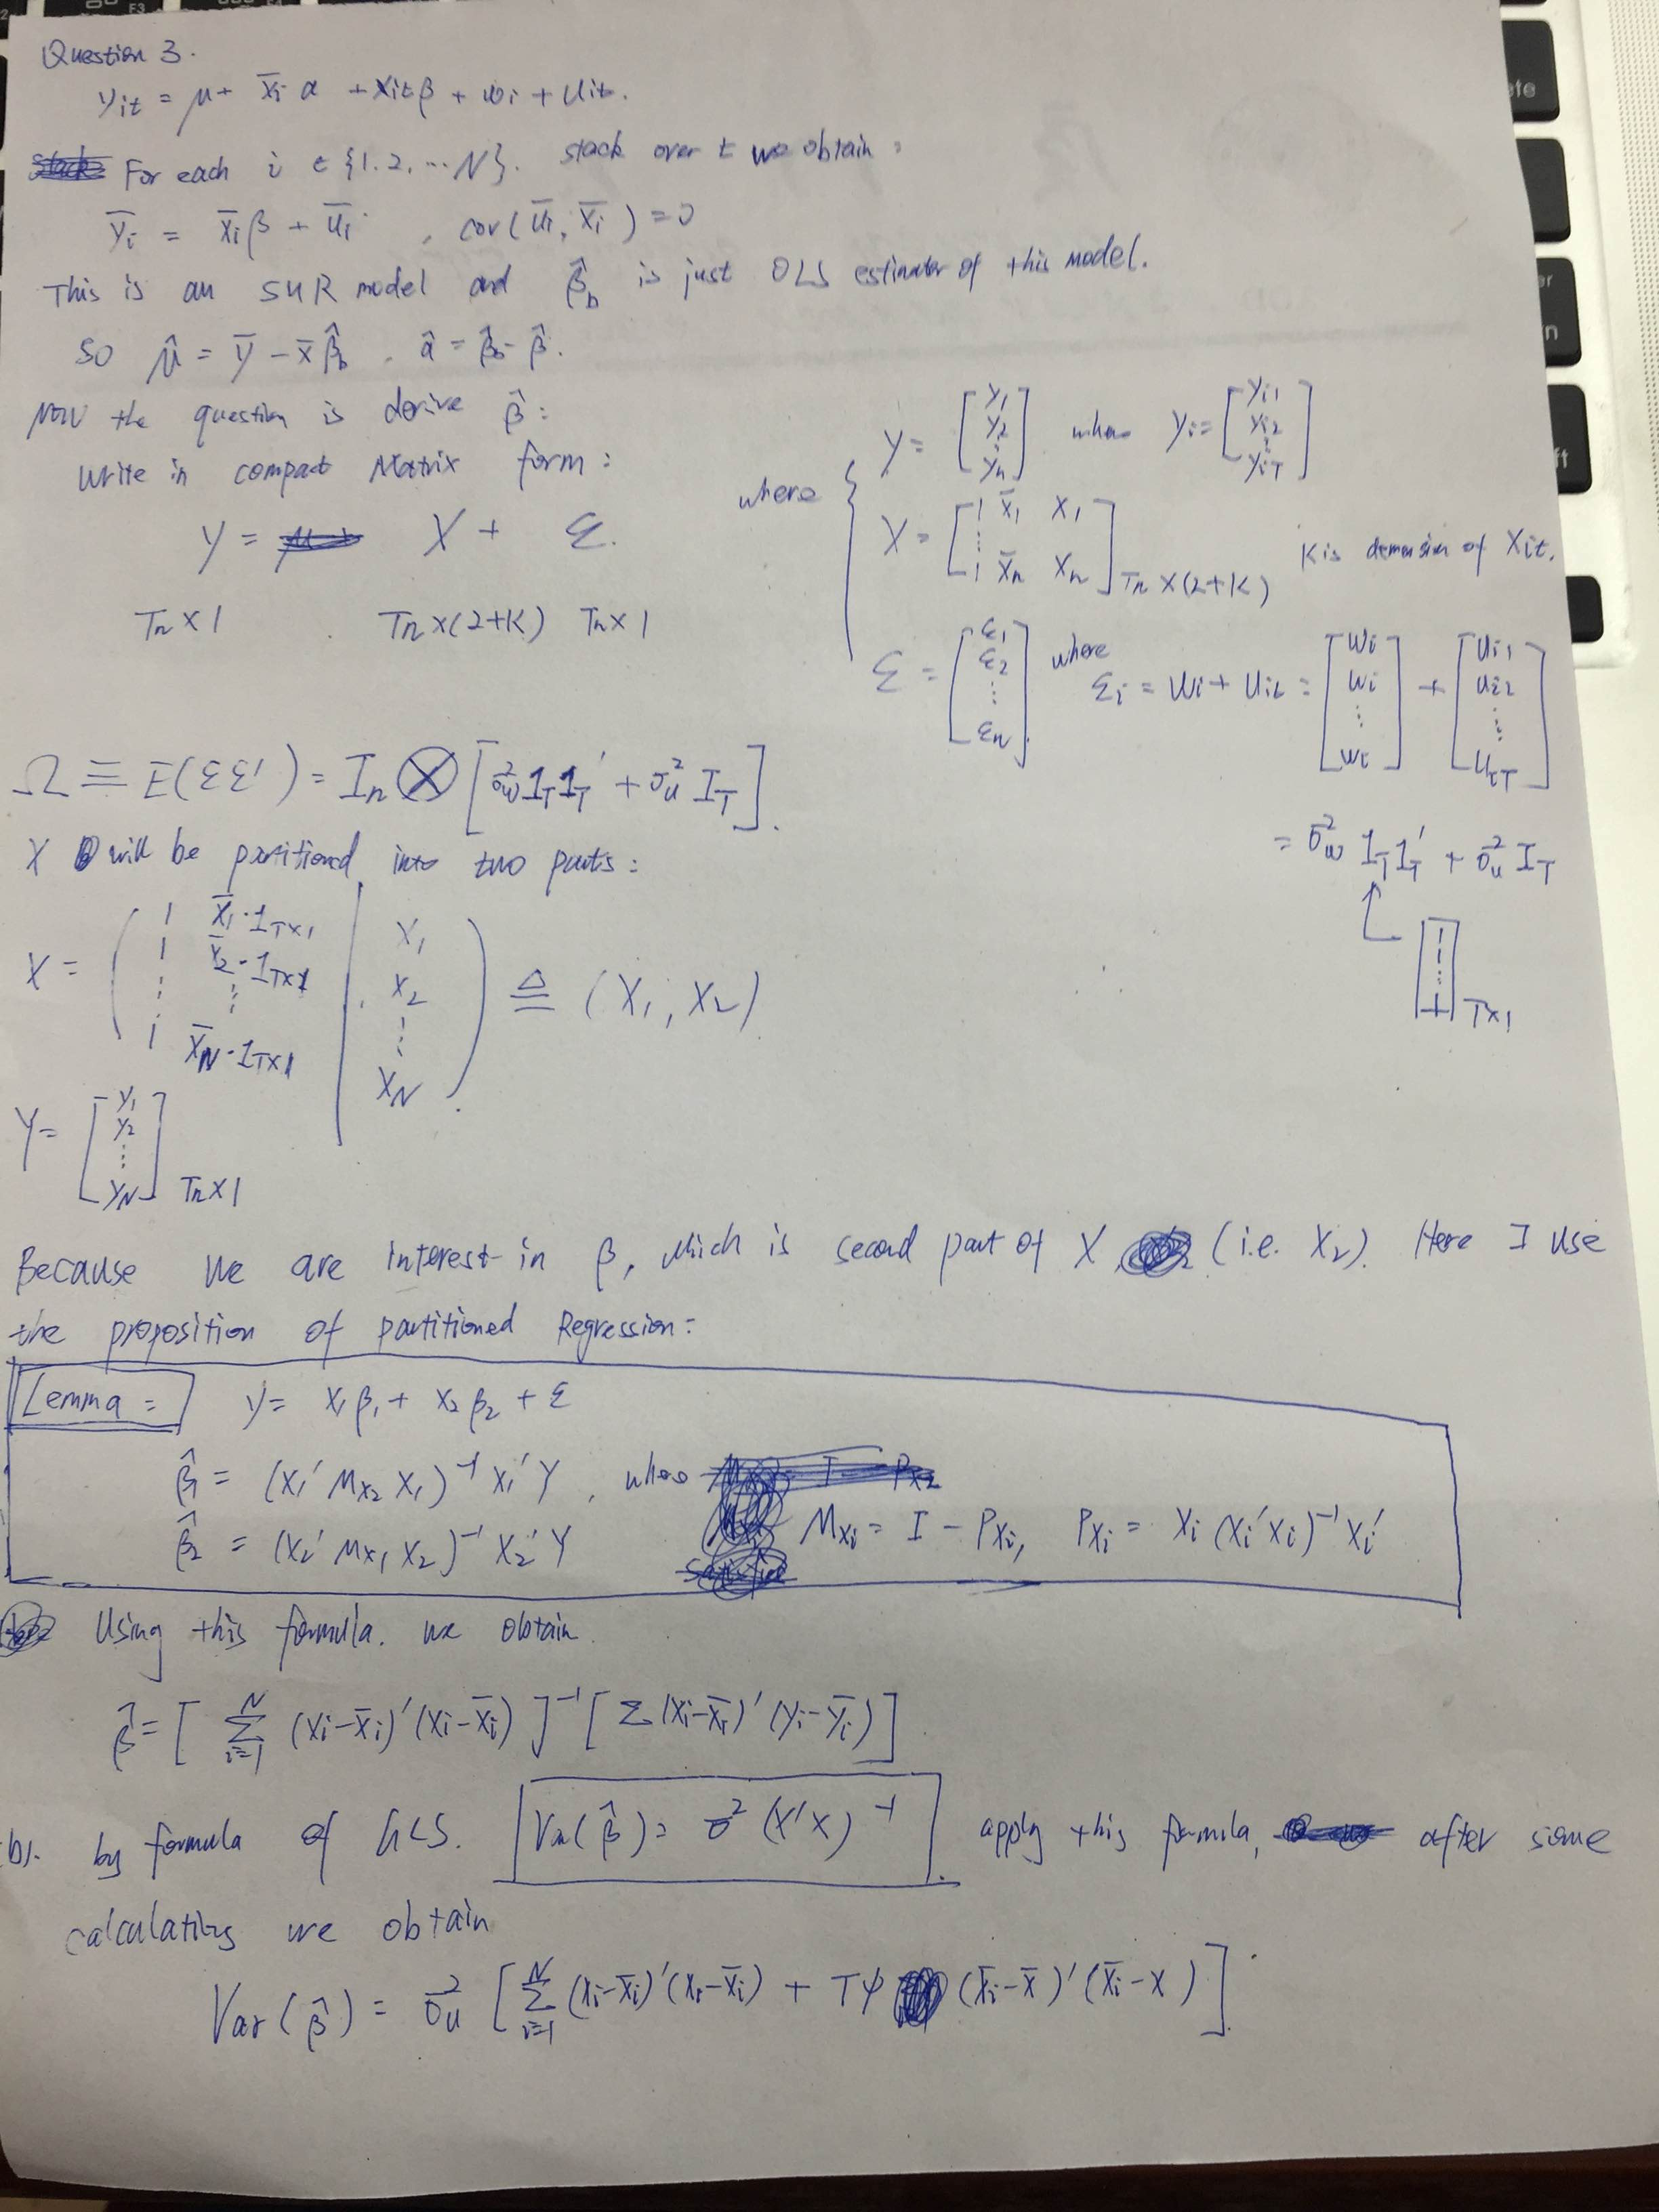
\includegraphics[width=1\linewidth]{Q3}
\caption{}
\label{fig:Q3}
\end{figure}




\end{document}